\documentclass{beamer} % slides

\mode<presentation>
{
  \usetheme{default} %Pittsburgh, default, boxes
  \setbeamertemplate{navigation symbols}{}
  \setbeamercovered{transparent}
  \setbeamersize
  {
    text margin left = 1.0em,
    text margin right = 1.0em
  }
  \setbeamercolor{section in toc}{fg=red}
  \setbeamercolor{section in toc shaded}{fg=structure}
  \setbeamertemplate{section in toc shaded}[default][100]
}

\usepackage[T1]{fontenc}
\usepackage[utf8]{inputenc}
\usepackage{textcomp}
\usepackage{lmodern}
\usepackage{hyperref}

\usepackage{amssymb}
\usepackage{latexsym}
\usepackage{stmaryrd}
\usepackage{extarrows}

\graphicspath{{figures/}}

\usepackage{tikz}
\usetikzlibrary{positioning,chains,matrix,shapes.arrows,scopes,
                shapes.misc,arrows,automata,calc,decorations.markings}
\everymath{\displaystyle}
\usepackage{pgf}

\tikzset{onslide/.code args={<#1>#2}{%
  \only<#1>{\pgfkeysalso{#2}} % \pgfkeysalso doesn't change the path
}}

\tikzset{dimmedmarker/.code args={<#1> then <#2>}{%
  \alt<#1,#2>
  {
    \tikzstyle{marker} = [draw]
    \alt<#2>
    {\pgfkeysalso{->,red!80,draw opacity=.15}}
    {\pgfkeysalso{->,red!80,draw opacity=.50}}
  }
  {
    \tikzstyle{marker} = [draw=none]}
}}

\tikzset{zdimmedmarker/.code args={<#1> then <#2>}{%
  \alt<#1,#2>
  {
    \tikzstyle{marker} = [draw]
    \alt<#2>
    {\pgfkeysalso{->,blue!80,draw opacity=.15}}
    {\pgfkeysalso{->,blue!80,draw opacity=.50}}
  }
  {
    \tikzstyle{marker} = [draw=none]}
}}

\tikzstyle{every picture}+=[remember picture]
\tikzstyle{na} = [baseline=-.5ex]
\tikzstyle{ln} = [baseline,every node/.style={anchor=base,inner sep=0}]
\tikzstyle{lm} = [baseline,every node/.style={anchor=base}]

\tikzstyle{weak} =
  [decoration={markings,
               mark=at position -.6mm with {\draw[fill=white] circle (.6mm);},
               mark=at position -1.1mm with {\arrow{latex}},
              }, postaction={decorate}]

\tikzstyle{strong} =
  [decoration={markings,
               mark=at position .6mm with {\draw[fill=white] circle (.6mm);},
                  }, postaction={decorate}, -latex]

% 1 - width (e.g., .95\textwidth); 2 - image name/path
\newenvironment{hgraphicscope}[2]
  {
    \node[anchor=south west,inner sep=0] (image) at (0,0)
       {\includegraphics[width=#1]{#2}};
    \begin{scope}
    \tikzset{every node/.style={}, every path/.style={}}
    \clip (image.south west) rectangle (image.north east);
    \path let \p1=(image.south east) in (\y1, \x1) coordinate (ylimit);
    \end{scope}
    \begin{scope}[x={(image.south east)},y={(ylimit)},scale=0.1,]
  }
  {
    \end{scope}
  }

%---  }-}2------------------------------------------------------------

\newcommand{\ipause}{\onslide+<+(1)->}
\newcommand{\makepoint}[1]{\textcolor{structure}{\textbf{#1}}}

% Useful slide macros

\newcommand<>{\blue}[1]{{\color#2{blue}{#1}}}
\newcommand<>{\green}[1]{{\color#2{green}{#1}}}
\newcommand<>{\red}[1]{{\color#2{red}{#1}}}
\newcommand<>{\violet}[1]{{\color#2{violet}{#1}}}
\newcommand<>{\gray}[1]{{\color#2{gray}{#1}}}

\usepackage[final,formats]{listings}
%\lstset{language=<...>,basicstyle=\sffamily}

\lstdefinelanguage{zelus}
   {morekeywords={
	let,in,rec,where,end,if,then,else,do,done,run,
	open,
	fun,node,hybrid,
	match,with,automaton,emit,
	pre,when,whenot,fby,merge,on,clock,
	or,and,not,as,mod,
	unless,until,continue,reset,every,await,
	init,der,type,last,
	period,local,present
    },
    sensitive=true,
    morecomment=[n]{(*}{*)},
    morestring=[b]",
    mathescape=true,
    escapechar=\%,
    columns=fullflexible,
    keepspaces=true,
    basicstyle=\sffamily\footnotesize,
    keywordstyle=\blue,
    xleftmargin=0em,
    literate={->}{{$\rightarrow$}}1
             {'a}{{$\alpha$}}1
             {'b}{{$\beta$}}1
             {_1}{{$_1$ }}1
             {_2}{{$_2$ }}1
             {_3}{{$_3$ }}1
             {_4}{{$_3$ }}1
             {_5}{{$_3$ }}1
             {_i}{{$_i$ }}1
             {~f}{{$f$}}1
             {...}{{$\ldots$}}1
             {~>}{{$\leadsto$}}1,
    }
%    belowskip=0em,

\lstnewenvironment{lst-zelus}[1]
    {\lstset{language=zelus,basicstyle=\sffamily#1}}
    {}

%int boolean float char string
%sig static

\newcommand{\zl}[1]{%
    \mbox{\lstinline[language=zelus,columns=fullflexible]{#1}}}

\newcommand{\zlt}[1]{%
    \mbox{\lstinline[language=zelus,columns=fullflexible,
                     basicstyle=\tiny,keywordstyle=\bfseries]{#1}}}

\lstdefinelanguage{zelusoutput}
   {morekeywords={val},
    sensitive=true,
    morecomment=[n]{(*}{*)},
    morestring=[b]",
    mathescape=true,
    columns=fullflexible,
    basicstyle=\sffamily\footnotesize,
    literate={->}{{$\rightarrow$}}1
             {-A>}{{$\stackrel{\mathtt{A}}{\rightarrow}$}}1
             {-C>}{{$\stackrel{\mathtt{C}}{\rightarrow}$}}1
             {-D>}{{$\stackrel{\mathtt{D}}{\rightarrow}$}}1
             {'a}{{$\alpha$}}1
             {'b}{{$\beta$}}1
             {'c}{{$\gamma$}}1
             {'d}{{$\delta$}}1
             {*}{{$\times$}}1
             {=>}{{$\Rightarrow$}}1
             {~>}{{$\leadsto$}}1,
    }
%    belowskip=0em,

\lstnewenvironment{lst-zelusoutput}
    {\lstset{language=zelusoutput}}
    {}

\newcommand{\zlo}[1]{%
    \mbox{\lstinline[language=zelusoutput,columns=fullflexible]{#1}}}



%--   }-}1%%%%%%%%%%%%%%%%%%%%%%%%%%%%%%%%%%%%%%%%%%%%%%%%%%%%%%%%%%%%

\pgfdeclareimage[height=1.5cm]{inria-logo}{inria-en.pdf}
\pgfdeclareimage[height=1.7cm]{ens-logo}{ens.pdf}

\title{The crazy fly}
\author{Timothy Bourke$^{1,2}$
\and Marc Pouzet$^{3,2,1}$}
\institute{
  1. INRIA Paris-Rocquencourt
  \and
  2. École normale supérieure (DI)
  \and
  3. Universit\'e Pierre et Marie Curie
  \\[2.0em]
  \url{http://www.di.ens.fr/ParkasTeam.html}
  \\[2.5em]
  %\pgfuseimage{inria-logo}
  %\hspace{3em}\raisebox{-.1cm}{\pgfuseimage{ens-logo}}
  }
\date{Synchron 2013, November 19, Daghstuhl, Germany}

\begin{document}

\begin{frame} %{-{1 title page
  \titlepage
\end{frame}

%--   }-}1%%%%%%%%%%%%%%%%%%%%%%%%%%%%%%%%%%%%%%%%%%%%%%%%%%%%%%%%%%%%

\begin{frame}{A very fast fly} %{-{1

  \begin{tikzpicture}

    \clip (-6,-4.2) [rounded corners]rectangle (6,4.2);

    \node at (0,0) {
      \includegraphics[width=\textwidth,trim=0 0 300 0,clip]{spain.pdf}};

    \ipause
    \draw[fill,white,opacity=.5] (-6,-4.2) rectangle (6,4.2);

    \coordinate (girona) at (0.72,3.72);
    \coordinate (barcelona) at (-5.62,-4.02);

    \draw[very thick,blue,latex-latex]
      ([xshift=1.5cm]barcelona -| girona)
        node[right] {Barcelona}
        -- node[right] {100km}
      ([xshift=1.5cm]girona)
        node[right] {Girona};

    \ipause

    \node[above right] (redcar) at ([xshift=-10]barcelona)
      {\includegraphics[width=2cm,angle=50]{redcar.pdf}};
    \node[right=.0cm of redcar,fill=white,rounded corners,text=red]{car$_1$ 
    = 50km/hr};

    \ipause

    \node[below] (greencar) at ([xshift=-10,yshift=5]girona)
      {\includegraphics[width=2cm,angle=20]{greencar.pdf}};
    \node[below=0cm of greencar,fill=white,rounded 
    corners,text=green]{car$_2$ = -50km/hr};

    \ipause

    \node[above] (fly) at (redcar)
      {\includegraphics[width=2cm,angle=40]{fly.pdf}};

    \node[right=0cm of fly,fill=white,text=black,text width=12em,rounded 
    corners]{\blue{fly = 80km/hr}\\changes direction whenever it reaches a 
    car};

  \end{tikzpicture}

\end{frame}
%--   }-}1%%%%%%%%%%%%%%%%%%%%%%%%%%%%%%%%%%%%%%%%%%%%%%%%%%%%%%%%%%%%

\begin{frame}{A very fast fly} %{-{1

  \begin{block}{The usual questions}
  \begin{enumerate}

  \item How far has the fly traveled when the two cars meet?

  \item How many zig-zags does the fly do during this period?

  \end{enumerate}
  \end{block}

  \bigskip
  \ipause

  \begin{block}{Extra credit (Thanks to Rafel Cases and Jordi Cortadella)}

  \begin{enumerate}
  \item Where will the fly be when the two cars reach their destinations?
  \end{enumerate}

  \end{block}

\end{frame}
%--   }-}1%%%%%%%%%%%%%%%%%%%%%%%%%%%%%%%%%%%%%%%%%%%%%%%%%%%%%%%%%%%%

\begin{frame}{Simulink model} %{-{1

  \begin{tikzpicture}

    \clip (-6.1,-3.4) [rounded corners]rectangle (6.1,3.3);

    \node at (0,0) {
      \includegraphics[width=6.8cm,angle=-90]{cantharide-sys-nohit.pdf}};
    \fill[white] (5.1,-2.56) rectangle (5.8,-2.45);

    \ipause
    \node[above right] (redcar) at (-5.8,.35)
      {\includegraphics[width=.7cm,angle=0]{redcar.pdf}};
    \node[above right] (greencar) at (-4.7,-.5)
      {\includegraphics[width=.7cm,angle=0]{greencar.pdf}};
    \node[above right] (fly) at (-5.3,-1.6)
      {\includegraphics[width=.7cm,angle=0]{fly.pdf}};

    \ipause

    \draw[red,very thick,->] (5.75,-1.8)
      node[left,red] {zigzags?} -- +(0,-.5);

  \end{tikzpicture}

\end{frame}
%--   }-}1%%%%%%%%%%%%%%%%%%%%%%%%%%%%%%%%%%%%%%%%%%%%%%%%%%%%%%%%%%%%

\begin{frame}{Simulink Results} %{-{1

  \begin{tikzpicture}

    \clip (-6.1,-3.4) [rounded corners]rectangle (6.1,3.6);

    \node at (0,0) {
      \includegraphics[width=.95\textwidth]{simulink-nohit.pdf}};

    \node[above right] (redcar) at (-5.70,-3.1)
      {\includegraphics[width=.7cm,angle=90]{redcar.pdf}};
    \node[above right] (greencar) at (-5.75,2.5)
      {\includegraphics[width=.7cm,angle=90]{greencar.pdf}};
    \node[below left] at (-5.0,-3.0) {\tiny{Barcelona}};
    \node[below left] at (-5.0,3.7) {\tiny{Girona}};
    \node[above right] (fly) at (-4.4,-2.2)
      {\includegraphics[width=.7cm,angle=0]{fly.pdf}};

  \end{tikzpicture}

  \bigskip
  \centerline{\gray{(Simulink R2012a: ode45, relative tolerance = 1e-3)}}

\end{frame}
%--   }-}1%%%%%%%%%%%%%%%%%%%%%%%%%%%%%%%%%%%%%%%%%%%%%%%%%%%%%%%%%%%%

\begin{frame}{Simulink model} %{-{1

  \begin{tikzpicture}

    \clip (-6.1,-3.4) [rounded corners]rectangle (6.1,3.3);

    \node at (0,0) {
      \includegraphics[width=6.8cm,angle=-90]{cantharide-sys-nohit.pdf}};
    %\fill[white] (5.1,-2.56) rectangle (5.8,-2.45);

    \node[above right] (redcar) at (-5.8,.35)
      {\includegraphics[width=.7cm,angle=0]{redcar.pdf}};
    \node[above right] (greencar) at (-4.7,-.5)
      {\includegraphics[width=.7cm,angle=0]{greencar.pdf}};
    \node[above right] (fly) at (-5.3,-1.6)
      {\includegraphics[width=.7cm,angle=0]{fly.pdf}};

    \draw[red,very thick,->] (5.75,-1.8)
      node[left,red] {zigzags} -- +(0,-.5);

  \end{tikzpicture}

\end{frame}
%--   }-}1%%%%%%%%%%%%%%%%%%%%%%%%%%%%%%%%%%%%%%%%%%%%%%%%%%%%%%%%%%%%

\begin{frame}{Simulink model (with more zero-crossings)} %{-{1

  \begin{tikzpicture}

    \clip (-6.1,-3.4) [rounded corners]rectangle (6.1,3.3);

    \node at (0,0) {
      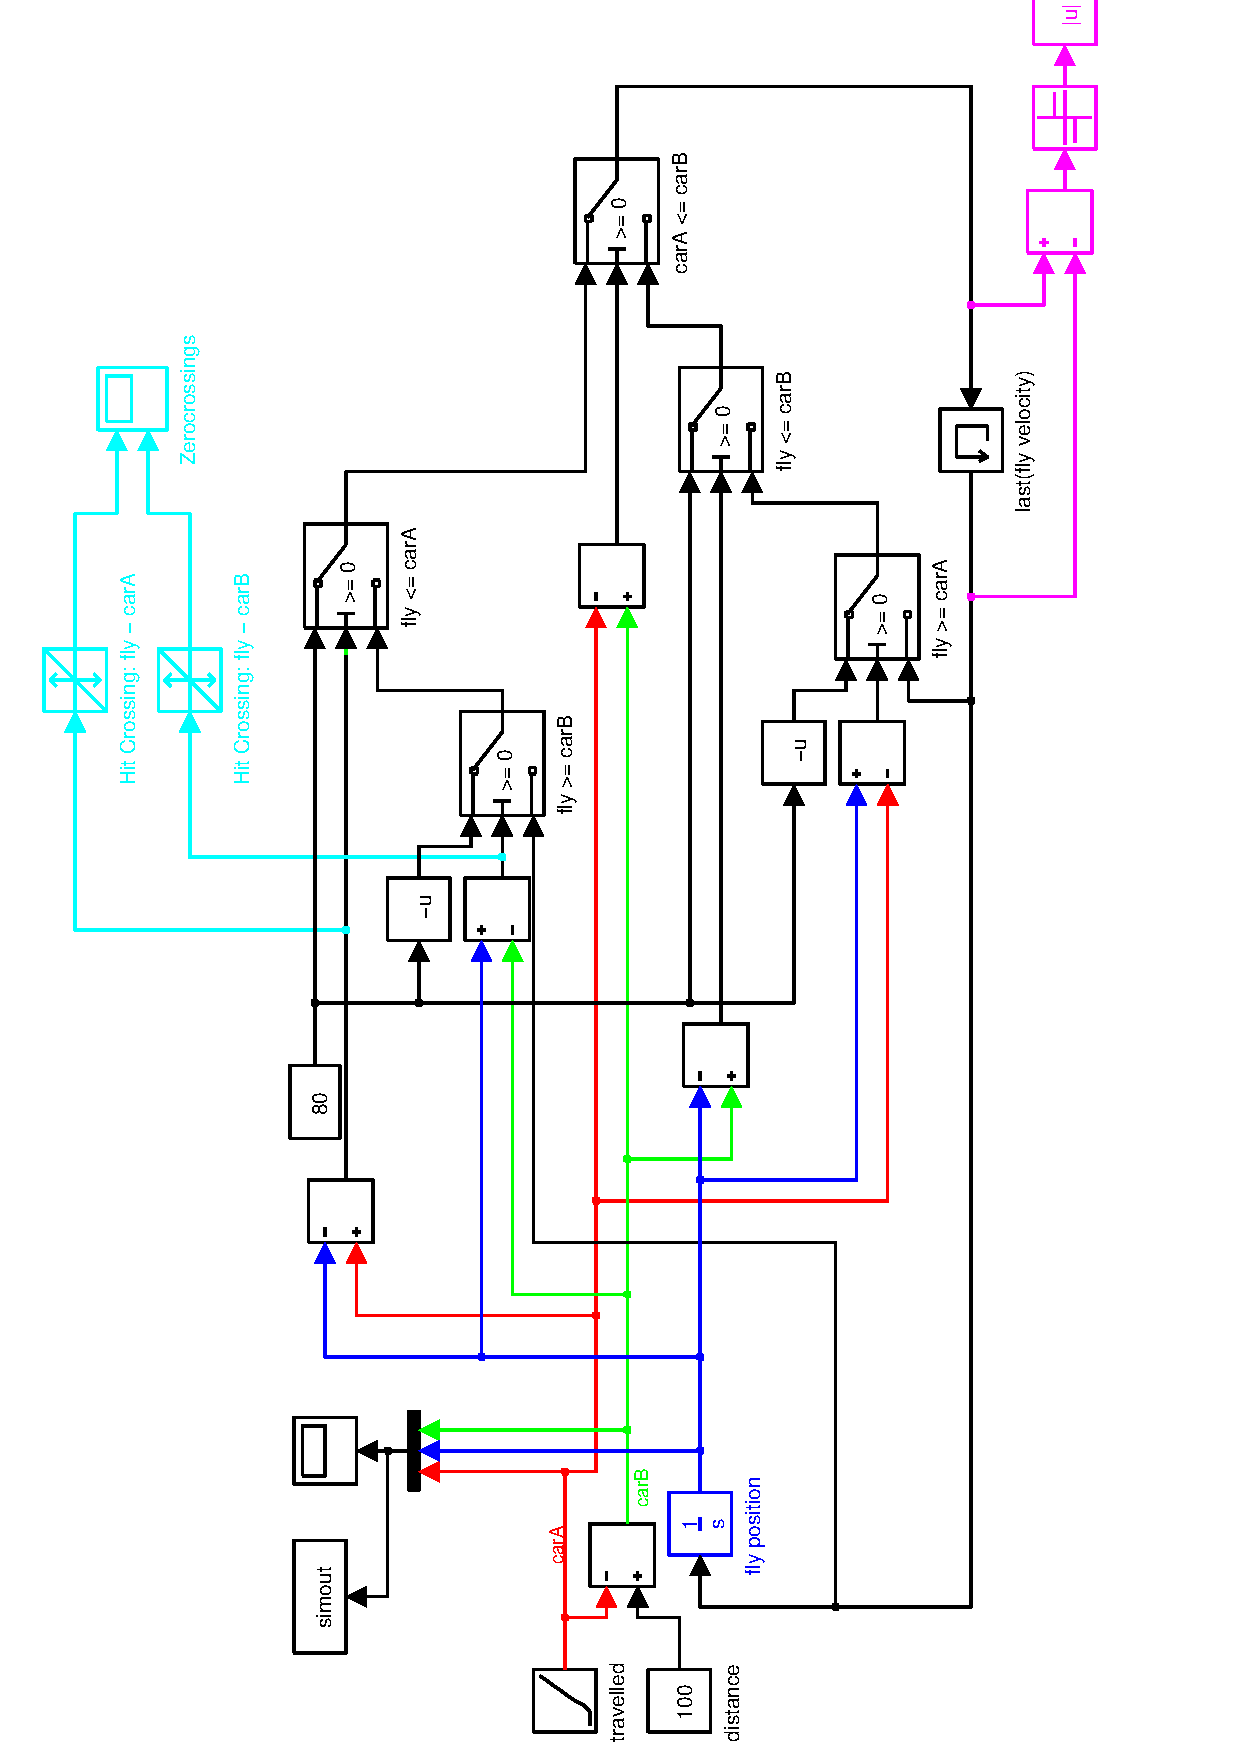
\includegraphics[width=6.8cm,angle=-90]{cantharide-sys.pdf}};
    \fill[white] (5.1,-2.56) rectangle (5.8,-2.45);

    \draw[red,very thick,->] (5.75,-1.8)
      node[left,red] {zigzags?} -- +(0,-.5);

    \node[above right] (redcar) at (-5.8,.35)
      {\includegraphics[width=.7cm,angle=0]{redcar.pdf}};
    \node[above right] (greencar) at (-4.7,-.5)
      {\includegraphics[width=.7cm,angle=0]{greencar.pdf}};
    \node[above right] (fly) at (-5.3,-1.6)
      {\includegraphics[width=.7cm,angle=0]{fly.pdf}};

  \end{tikzpicture}

\end{frame}
%--   }-}1%%%%%%%%%%%%%%%%%%%%%%%%%%%%%%%%%%%%%%%%%%%%%%%%%%%%%%%%%%%%

\begin{frame}{Simulink Results (with more zero-crossings)} %{-{1

  \begin{tikzpicture}

    \clip (-6.1,-3.4) [rounded corners]rectangle (6.1,3.6);

    \node at (0,0) {
      \includegraphics[width=.95\textwidth]{simulink.pdf}};

    \node[above right] (redcar) at (-5.70,-3.1)
      {\includegraphics[width=.7cm,angle=90]{redcar.pdf}};
    \node[above right] (greencar) at (-5.75,2.5)
      {\includegraphics[width=.7cm,angle=90]{greencar.pdf}};
    \node[below left] at (-5.0,-3.0) {\tiny{Barcelona}};
    \node[below left] at (-5.0,3.7) {\tiny{Girona}};
    \node[above right] (fly) at (-4.4,-2.2)
      {\includegraphics[width=.7cm,angle=0]{fly.pdf}};

    \ipause

    \node[fill=white] at (0,0) {
      \includegraphics[width=.5\textwidth]{simulink-zoom.pdf}};
    \node at (0,-2) {[0.9999999999999:1.0000000000001]};

  \end{tikzpicture}

  \bigskip
  \centerline{\gray{(Simulink R2012a: ode45, relative tolerance = 1e-3)}}

\end{frame}
%--   }-}1%%%%%%%%%%%%%%%%%%%%%%%%%%%%%%%%%%%%%%%%%%%%%%%%%%%%%%%%%%%%

\begin{frame}{Simulink model (with more zero-crossings)} %{-{1

  \begin{tikzpicture}

    \clip (-6.1,-3.4) [rounded corners]rectangle (6.1,3.3);

    \node at (0,0) {
      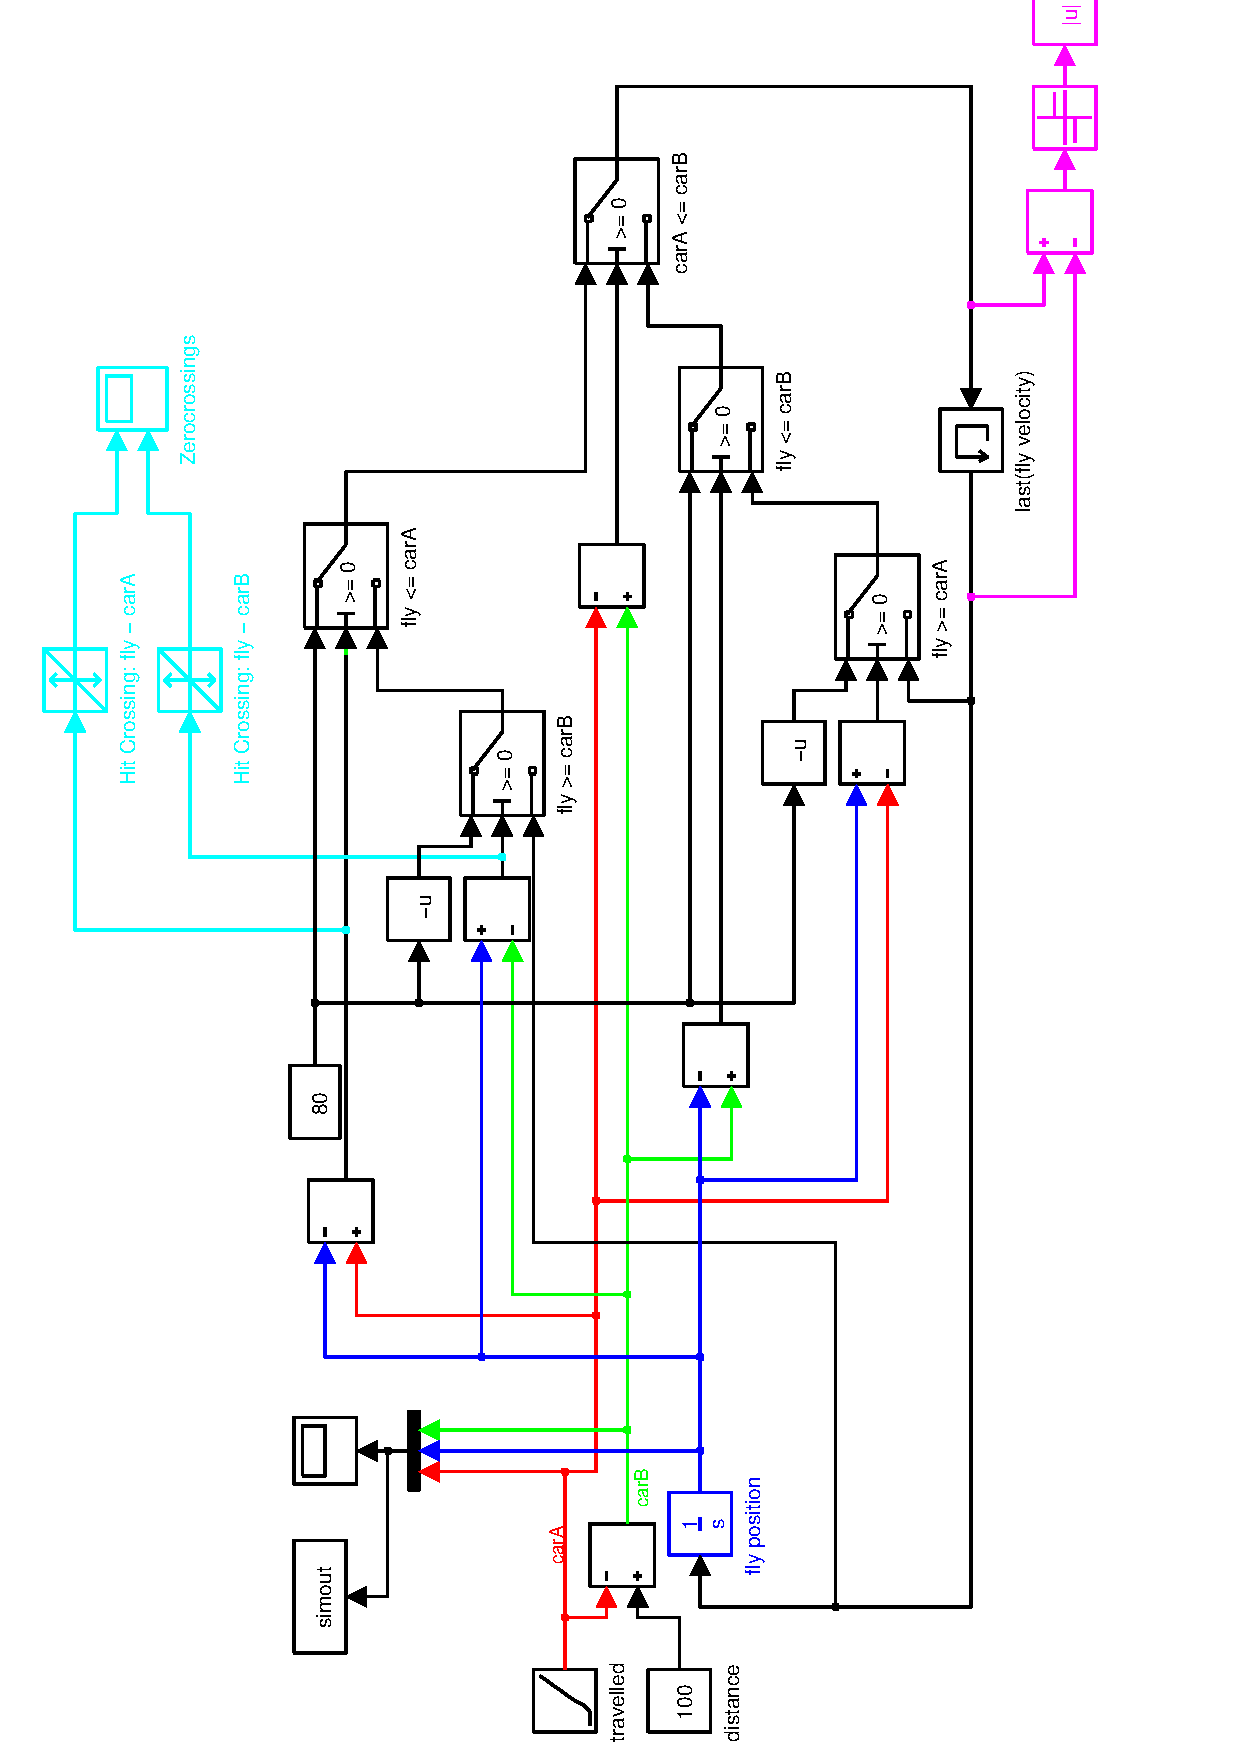
\includegraphics[width=6.8cm,angle=-90]{cantharide-sys.pdf}};
    %\fill[white] (5.1,-2.56) rectangle (5.8,-2.45);

    \draw[red,very thick,->] (5.75,-1.8)
      node[left,red] {zigzags} -- +(0,-.5);

    \node[above right] (redcar) at (-5.8,.35)
      {\includegraphics[width=.7cm,angle=0]{redcar.pdf}};
    \node[above right] (greencar) at (-4.7,-.5)
      {\includegraphics[width=.7cm,angle=0]{greencar.pdf}};
    \node[above right] (fly) at (-5.3,-1.6)
      {\includegraphics[width=.7cm,angle=0]{fly.pdf}};

  \end{tikzpicture}

\end{frame}
%--   }-}1%%%%%%%%%%%%%%%%%%%%%%%%%%%%%%%%%%%%%%%%%%%%%%%%%%%%%%%%%%%%

\begin{frame}{} %{-{1

  \centerline{\scalebox{10}{\Huge\red{42!}}}

\end{frame}

\begin{frame}{} %{-{1

  \centerline{\huge\blue{Let us try Z\'elus...}}

\end{frame}
%--   }-}1%%%%%%%%%%%%%%%%%%%%%%%%%%%%%%%%%%%%%%%%%%%%%%%%%%%%%%%%%%%%

\begin{frame}[fragile]{Zélus model~\footnote{\url{zelus.di.ens.fr}}}

\begin{lst-zelus}{\tiny}
let barcelona = 0.0
let girona = 100.0

let fly_velocity = 80.0
let car_velocity = 50.0

let hybrid model () =  (car1, car2, fly, zigzag, zeros) where
  rec der car1 = car_velocity      init barcelona
  and der car2 = -. car_velocity init girona
  and der fly = dir *. fly_velocity init barcelona
  and automaton
        | Above -> (* the line above the fly *) 
             do car_above = car2
             and car_below = car1
             until up(car1 -. car2) then Below
        | Below -> (* the line below *)
             do car_above = car1
             and car_below = car2
             done
        end
  and present 
         up (car_below -. fly) | up(fly -. car_above) -> 
           (* the fly changes her direction *)
           (* when she crosses the line below or the line above *)
           do dir = -. (last dir)
           and zeros = last zeros + 1
           and emit zigzag = ()
           done
  and init dir = 1.0
  and init zeros = 0
\end{lst-zelus}

\begin{tikzpicture}[overlay]
  \ipause

  \node[above right] (redcar) at (-.5,5.7)
    {\includegraphics[width=.7cm,angle=0]{redcar.pdf}};
  \node[above right] (greencar) at (4.5,5.4)
    {\includegraphics[width=.7cm,angle=0]{greencar.pdf}};
  \node[above right] (fly) at (-.5,5.0)
    {\includegraphics[width=.7cm,angle=0]{fly.pdf}};

  \ipause

  \draw[red,very thick,->] (4.0,6.8)
    node[right,red] {zigzags=48} -- +(0,-.3);

\end{tikzpicture}

\end{frame}
%--   }-}1%%%%%%%%%%%%%%%%%%%%%%%%%%%%%%%%%%%%%%%%%%%%%%%%%%%%%%%%%%%%

\begin{frame}{Zélus Results} %{-{1

  \begin{tikzpicture}

    \clip (-6.1,-3.4) [rounded corners]rectangle (6.1,3.6);

    \node at (0,0) {
      \includegraphics[width=.95\textwidth]{zelus.pdf}};

    \node[above right] (redcar) at (-5.70,-3.1)
      {\includegraphics[width=.7cm,angle=90]{redcar.pdf}};
    \node[above right] (greencar) at (-5.75,2.5)
      {\includegraphics[width=.7cm,angle=90]{greencar.pdf}};
    \node[below left] at (-5.0,-3.0) {\tiny{Barcelona}};
    \node[below left] at (-5.0,3.7) {\tiny{Girona}};
    \node[above right] (fly) at (-4.4,-2.2)
      {\includegraphics[width=.7cm,angle=0]{fly.pdf}};

    \ipause

    \node[fill=white] at (0,0) {
      \includegraphics[width=.5\textwidth]{zelus-zoom.pdf}};
    \node at (0,-2) {[0.9999999999999\violet{95}:1.0000000000000\violet{05}]};

  \end{tikzpicture}

  \bigskip
  \centerline{\gray{(Sundials CVODE with our custom Illinois implementation)}}

\end{frame}
%--   }-}1%%%%%%%%%%%%%%%%%%%%%%%%%%%%%%%%%%%%%%%%%%%%%%%%%%%%%%%%%%%%

\begin{frame}{Concluding remarks} % {-{1

\begin{block}{Simulink}
42 is the answer to ``The Ultimate Question of Life, the
Universe and Everything''~\footnote{cf Douglas Adams, The Hitchhiker's Guide
to the Galaxy.}. \red{Trop fort!}
\end{block}

\begin{block}{Well...}
\begin{itemize}
\item
All very well, but the problem is mathematically not well posed.
\item
The system is not well defined at the instant the cars pass each other.
\end{itemize}
\end{block}


\begin{block}{Question: should a hybrid modeler}
\begin{itemize}
\item
statically detect and reject such programs?
\item
stop with an error at runtime?\footnote{In the same way variable-step
integration fails when reaching a minimal horizon.}
\end{itemize}

\end{block}

\medskip

(Thanks to Rafel Cases, Jordi Cortadella, and Gérard Berry.)
 
\end{frame}

%--   }-}1%%%%%%%%%%%%%%%%%%%%%%%%%%%%%%%%%%%%%%%%%%%%%%%%%%%%%%%%%%%%


\end{document}

